\begin{enumerate}
	\item L'administrateur se connecte au site avec ses identifiant. 
	\item Un nouveau bouton de navigation apparait dans la bar de navigation. 
	\item L'administrateur clique sur le bouton \textit{Admin}
	\item Il sélectionne \textit{Nouvelle sessions} dans le menu déroulant. 
	\item L'administrateur atterris sur la page de création de session. 
	\item Il clique sur \textit{Génération auto}
	\item Un formulaire lui demandant sur combien d'année ainsi que quelle type de session il souhaite générer apparait.
	\item Il sélectionne les types de sessions qu'il souhaite générer.
	\item Il indique le nombre d'année voulus
	\item Il clique sur \textit{Je confirme la génération} 
\end{enumerate}

\vspace{\baselineskip}
\begin{figure}[h]
	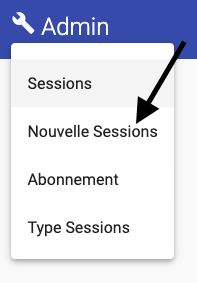
\includegraphics[width=0.4\textwidth,center]{Figures/us16-1}
	\caption{Menu de l'administrateur}
\end{figure}

\newpage
\begin{figure}[h]
	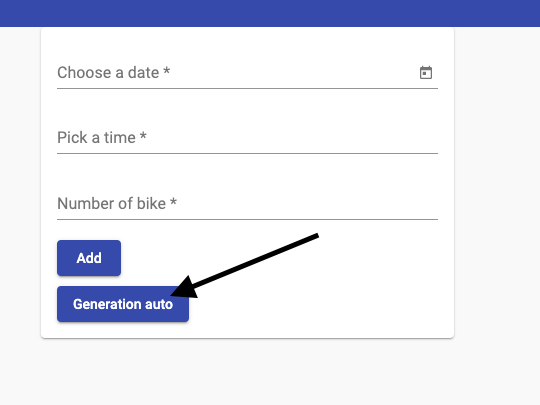
\includegraphics[width=0.4\textwidth,center]{Figures/us16-2}
	\caption{Bouton de génération automatique}
\end{figure}

\vspace{\baselineskip}
\begin{figure}[h]
	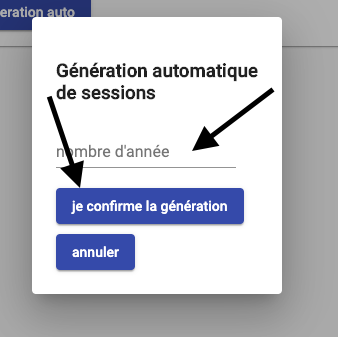
\includegraphics[width=0.3\textwidth,center]{Figures/us16-3}
	\caption{Formulaire pour le génération automatique de session}
\end{figure}


\subsubsection{Gestion des erreurs}
	\begin{itemize}
		\item La génération automatique suppose que tout les types de sessions on été préalablement configurer si ce n'est pas le cas une erreur apparaitra à la confirmation.
		\item Si une erreur se créer durant la génération elle est interrompus et un message d'erreur est afficher à l'administrateur.
	\end{itemize}
	
\newpage
\subsubsection{Diagramme de séquence}
	\begin{figure}[h]
		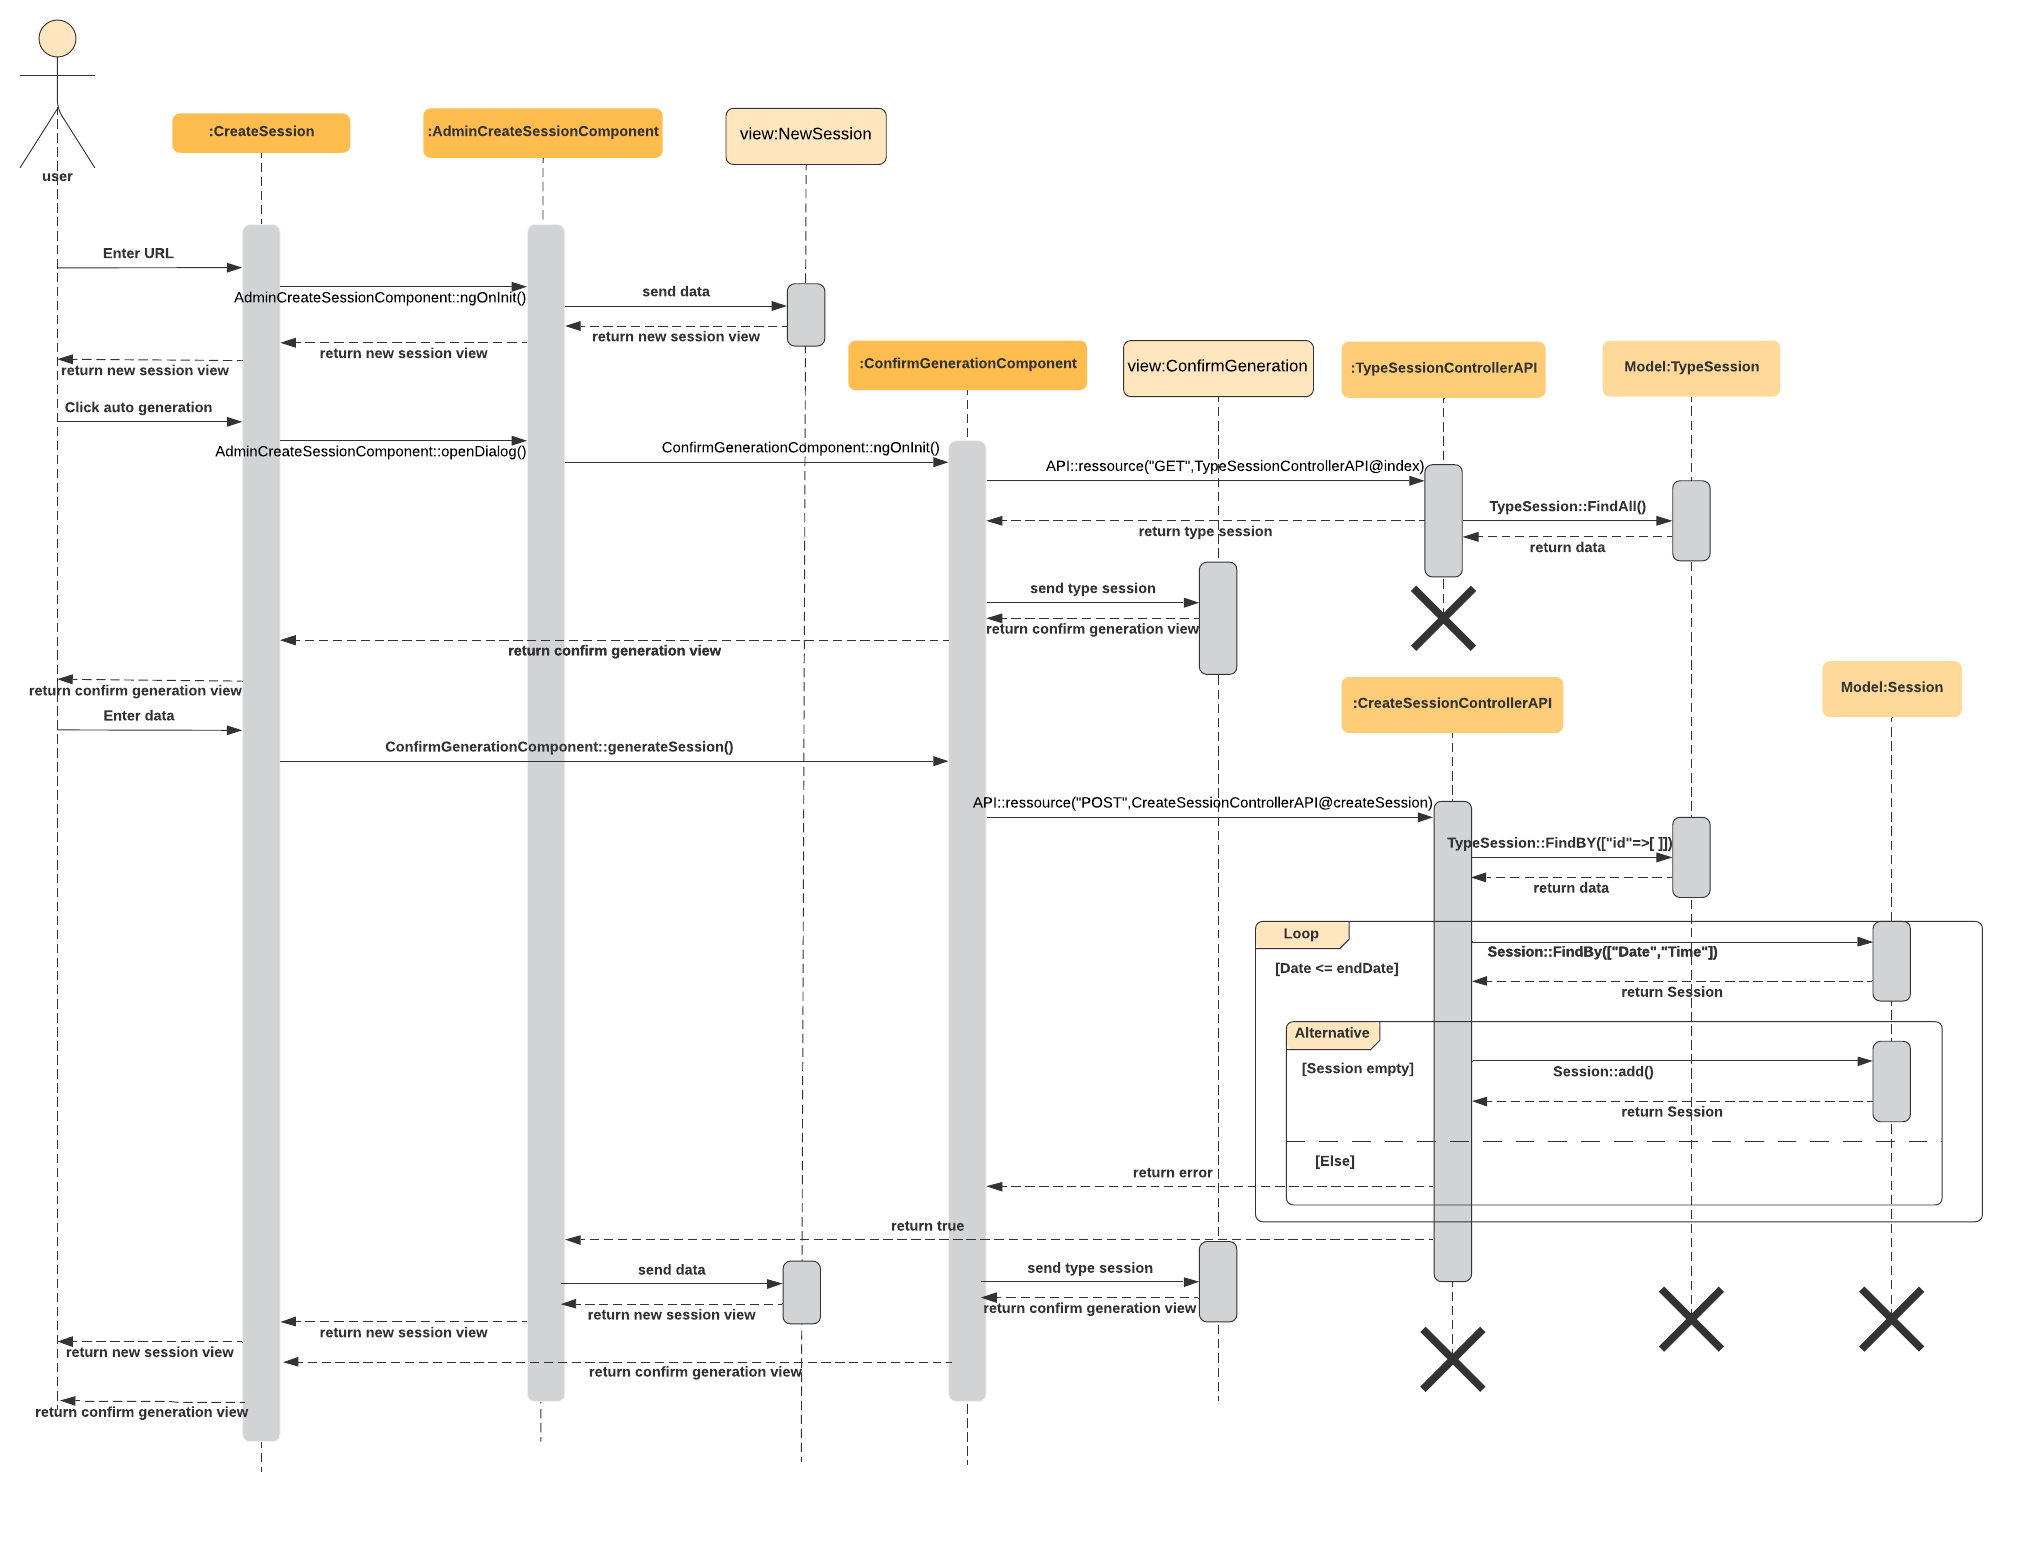
\includegraphics[width=\textwidth,center]{Diagramme/sequence-us16}
		\caption{Diagramme de séquence de la génération automatique de session}
	\end{figure}
	

\subsubsection{Script concernés}
	\begin{itemize}
		\item \Href{https://github.com/victorsmits/Aquabike/blob/master/backend/src/Entity/Session.php}{Session.php}
		\item \Href{https://github.com/victorsmits/Aquabike/blob/master/backend/src/Controller/API/CreateSessionControllerApi.php}{CreateSessionControllerApi.php}
		\item \Href{https://github.com/victorsmits/Aquabike/blob/master/frontend/src/app/admin-create-session/admin-create-session.component.ts}{admin-create-session.component.ts}
		\item \Href{https://github.com/victorsmits/Aquabike/blob/master/frontend/src/app/admin-create-session/admin-create-session.component.html}{admin-create-session.component.html}
	\end{itemize}